\chapter{Modelling Evolution of Life-history Traits}
\section{Modelling Adult Stage}
After modelling the larval stage and calibrating, I developed the model for the pupal and adult stage of \textit{Drosophila} life cycle. After the larval stage, surviving individuals go through the pupal stage, where some of them undergo pupal mortality. The adult stage includes randomly choosing surviving adults from all replicate vials of the pupal stage, matings, and inheritance of larval trait parameters from parents to offspring. Female is mated once with random male chosen (with replacement) from the adult population ($n$ = 2400) for simplicity. From all the offspring produced, eggs are chosen at random for the next generation with numbers respective to the crowding environment maintained.
\subsection{Pupal stage}
After collecting all the surviving individuals from the larval stage, a probability of death during the pupal stage is assigned to each survived larva. This probability is dependent on the amount of waste accumulated in the body while consuming food during the larval stage. This probability is given as:
\[P_{M}(i) = 1 - exp(-(W_{acum}(i) \cdot x_{3})^{2})\]
Here, \\
$P_{M}$: probability of dying during pupal stage; \\
$W_{acum}(i)$: waste accumulated by $i^{th}$ larva during larval stage; \\
$x_{3}$: scaling parameter.
\subsection{Fecundity}
After each mating, the number of eggs produced for a female is derived from the fecundity equation based on the model of \citep{tungComplexInteractionResource2019}. Fecundity is taken as a function of body size of the female and adult nutrition parameter (the amount of yeast provided). Fecundity of an $i^{th}$ female is given as:
\[Egg_{i} = Nut \cdot x_{4} \cdot \log{(x_{5} \cdot s_{i})}\]
Here, $s_{i}$: body size of the $i^{th}$ female; \\
$Egg_{i}$: number of eggs laid by the female in a mating; \\
$Nut$: adult nutrition i.e. the amount of yeast provided; \\
$x_{4}, x_{5}$: scaling parameters.
\subsection{Inheritance}
Larval trait parameters (initial feeding rate, efficiency, waste tolerance and critical size) are inherited from parents to offspring produced by each female using mid-parent value. The mid-parent value, i.e. the average of mother and father for each larval parameter of all offspring, is calculated. This mid-parent value is taken as a mean of a normal distribution with a fixed standard deviation for respective trait parameters. The standard deviation in this normal distribution determines the heritability of the mid-parent value, and it is considered to be different for each trait parameter. Trait parameters of the offspring are assigned as:
\[T_{i} \in N(mpv_{T}, \delta_{T})\]
Here, \\
$T_{i}$: trait parameter assigned to $i^{th}$ offspring from a mating; \\
$mpv_{T}$: mid-parent value of of the trait $T$ for a given mating; \\
$\delta_{T}$: heritability of mid-parent value of the trait $T$; \\
$N(mpv, \delta)$: normal distribution with $mpv$ as mean and $\delta$ as standard deviation.
\begin{figure}[p]
  \centering
  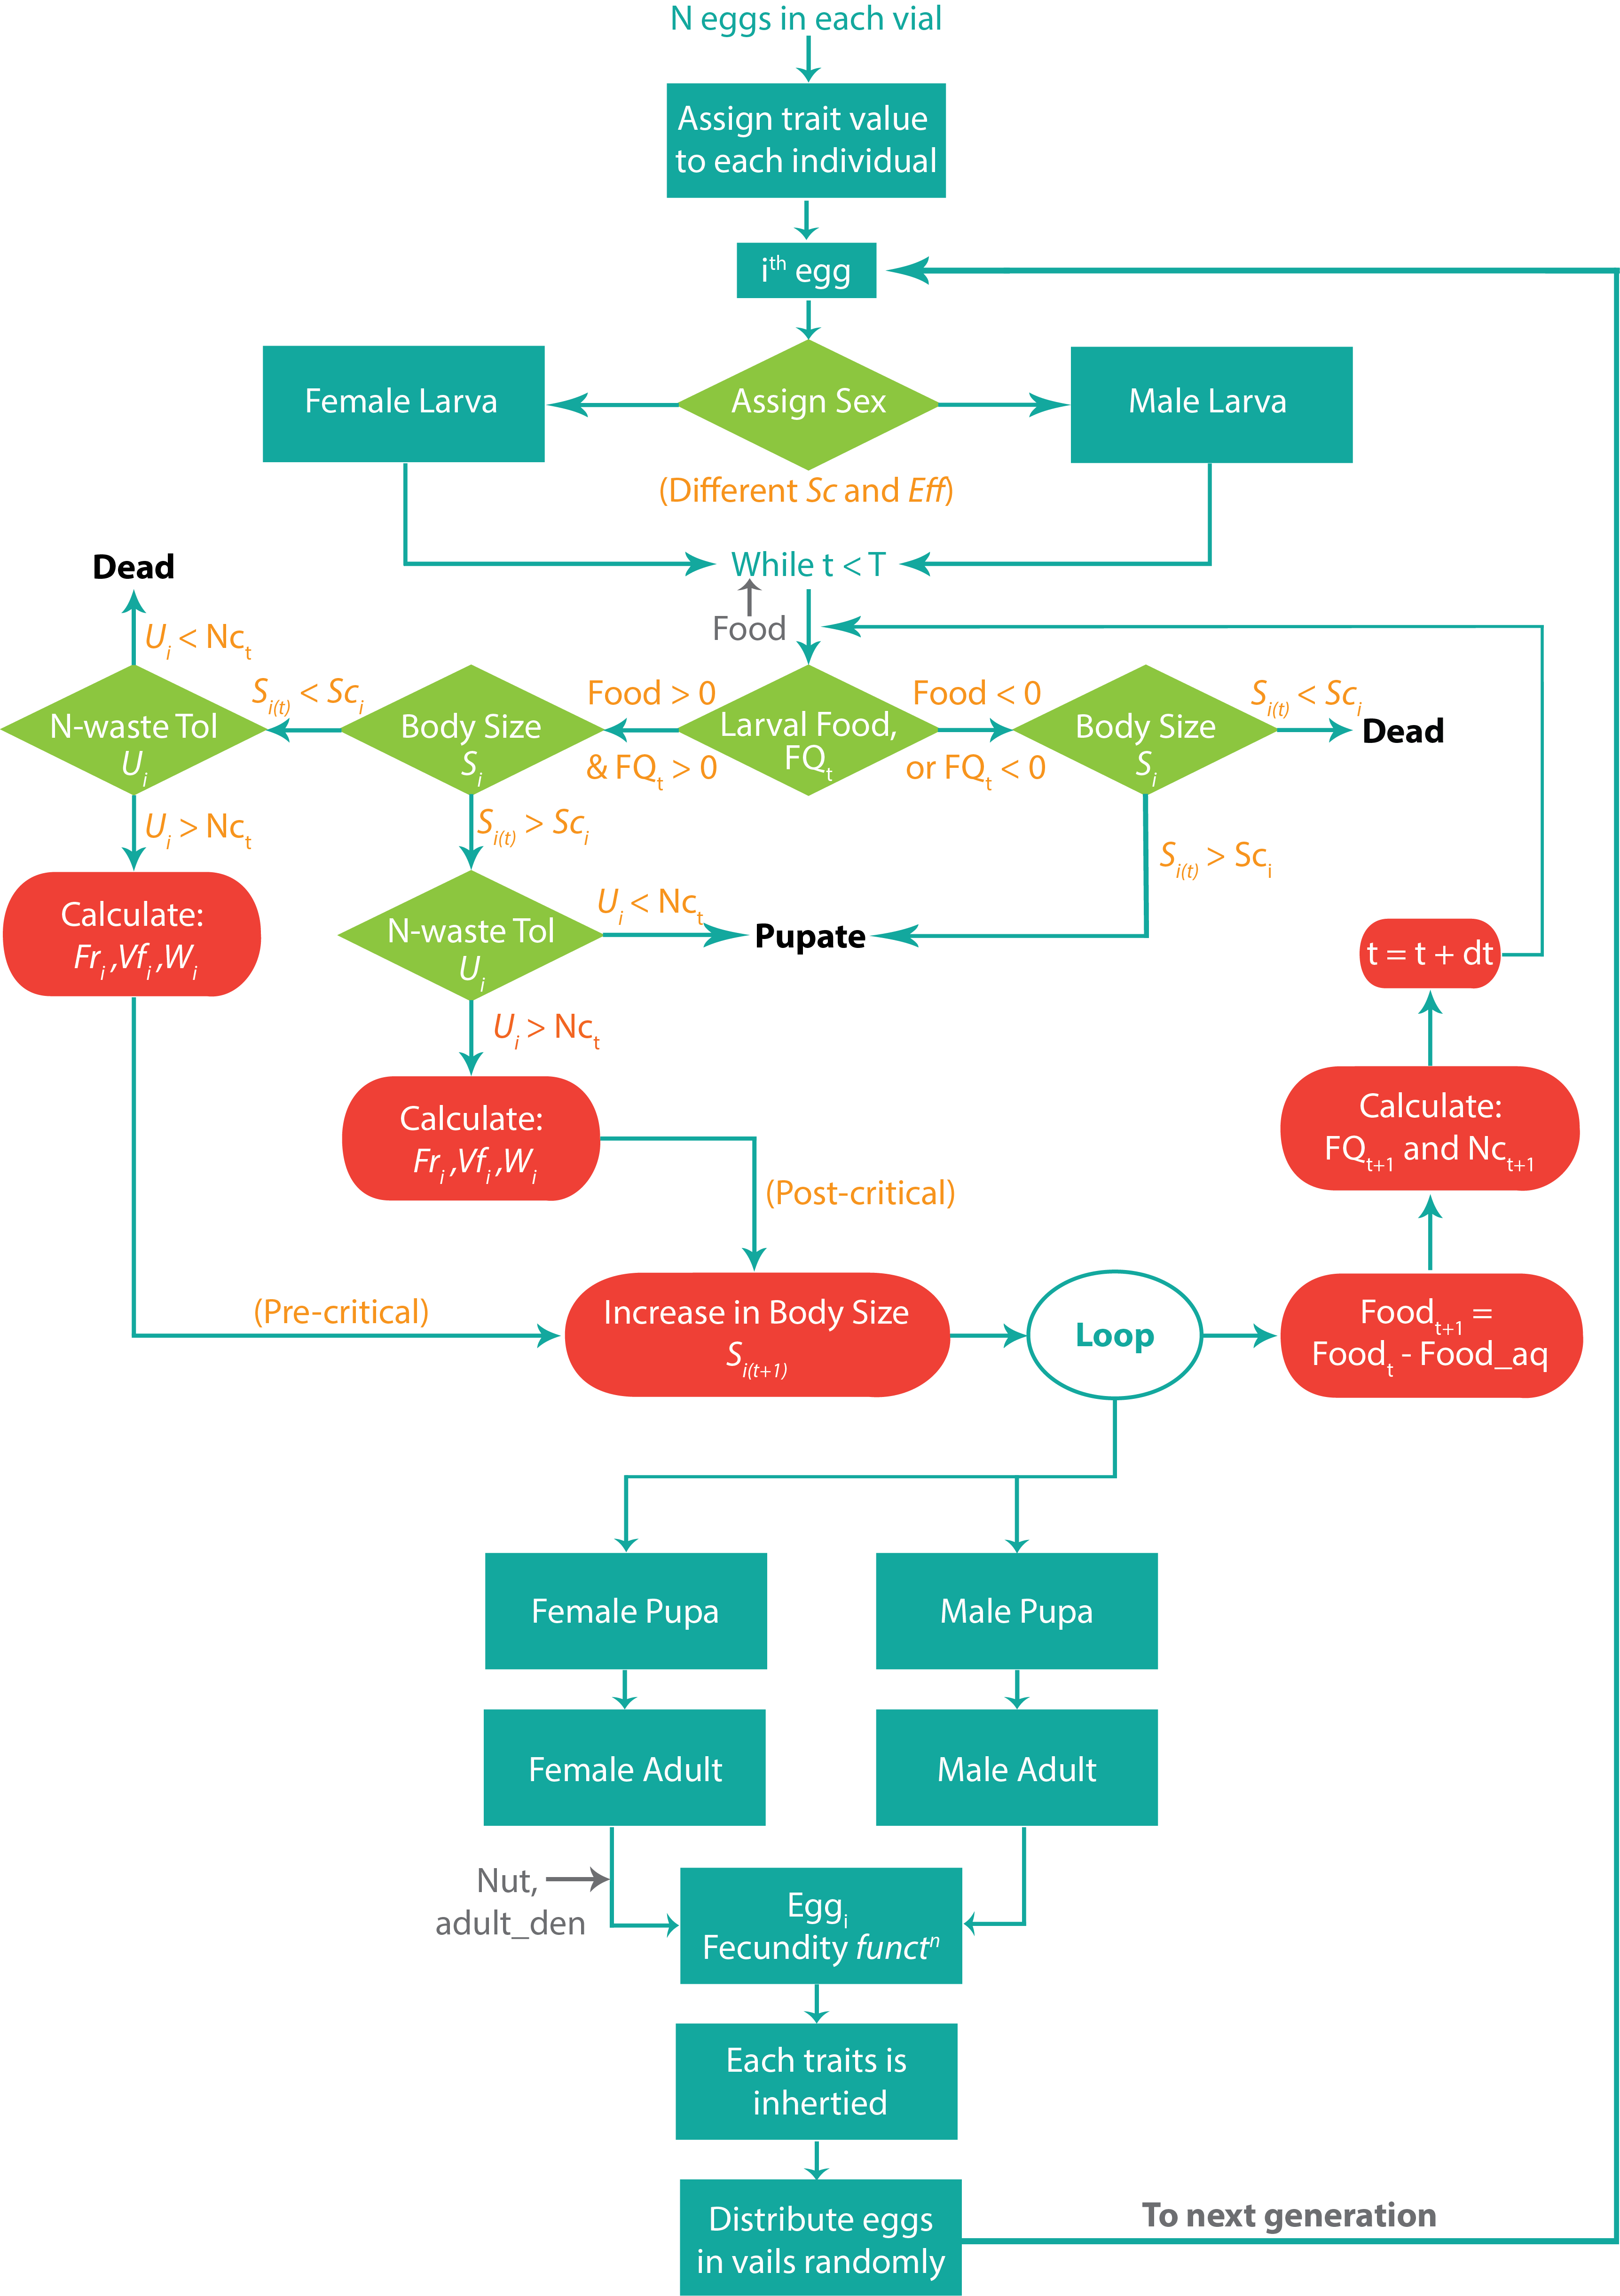
\includegraphics[trim= 0 0 0 0, clip, width= \textwidth]{C4/Figs/model}
  \caption{Complete flowchart of the model }
  \label{model}
\end{figure}

\clearpage
\section{Evolution of Larval Trait Parameters}
Using values for all parameters given in table~\ref{tab:scale_param} and table~\ref{tab:food_param}, the entire model is simulated for 100 generations with 10 replicates for MB, MCU and CCU cultures (see fig~\ref{model}). This first set of simluations on the evolutionary part is aimed at investigating differences in the evolution of competitive ability in MCU and CCU populations which have same larval density but different ecological dynamics. In the model, all larval trait parameters are taken from independent distribution, and there is no correlation between them (see table~\ref{tab:trait_value}). Timeseries for these traits of surviving adult individuals are plotted with 95$\%$ CI.\\ \\
In MB culture, being control population, none of the trait parameters evolve over time (see fig~\ref{fr} - ~\ref{wtol}). Initial feeding rate in high-density cultures increase over generations at a similar rate, but initial feeding rate is higher always in CCU culture than in MCU culture. Efficiency shows a similar trend in high-density cultures, i.e. increase over generations at a similar rate which is always higher in CCU culture always than in MCU culture. Critical size in CCU culture is always lower than in MCU culture. Waste tolerance does not evolve in all of the culture populations since there is no significant change in waste tolerance value.
\begin{figure}[h]
  \centering
  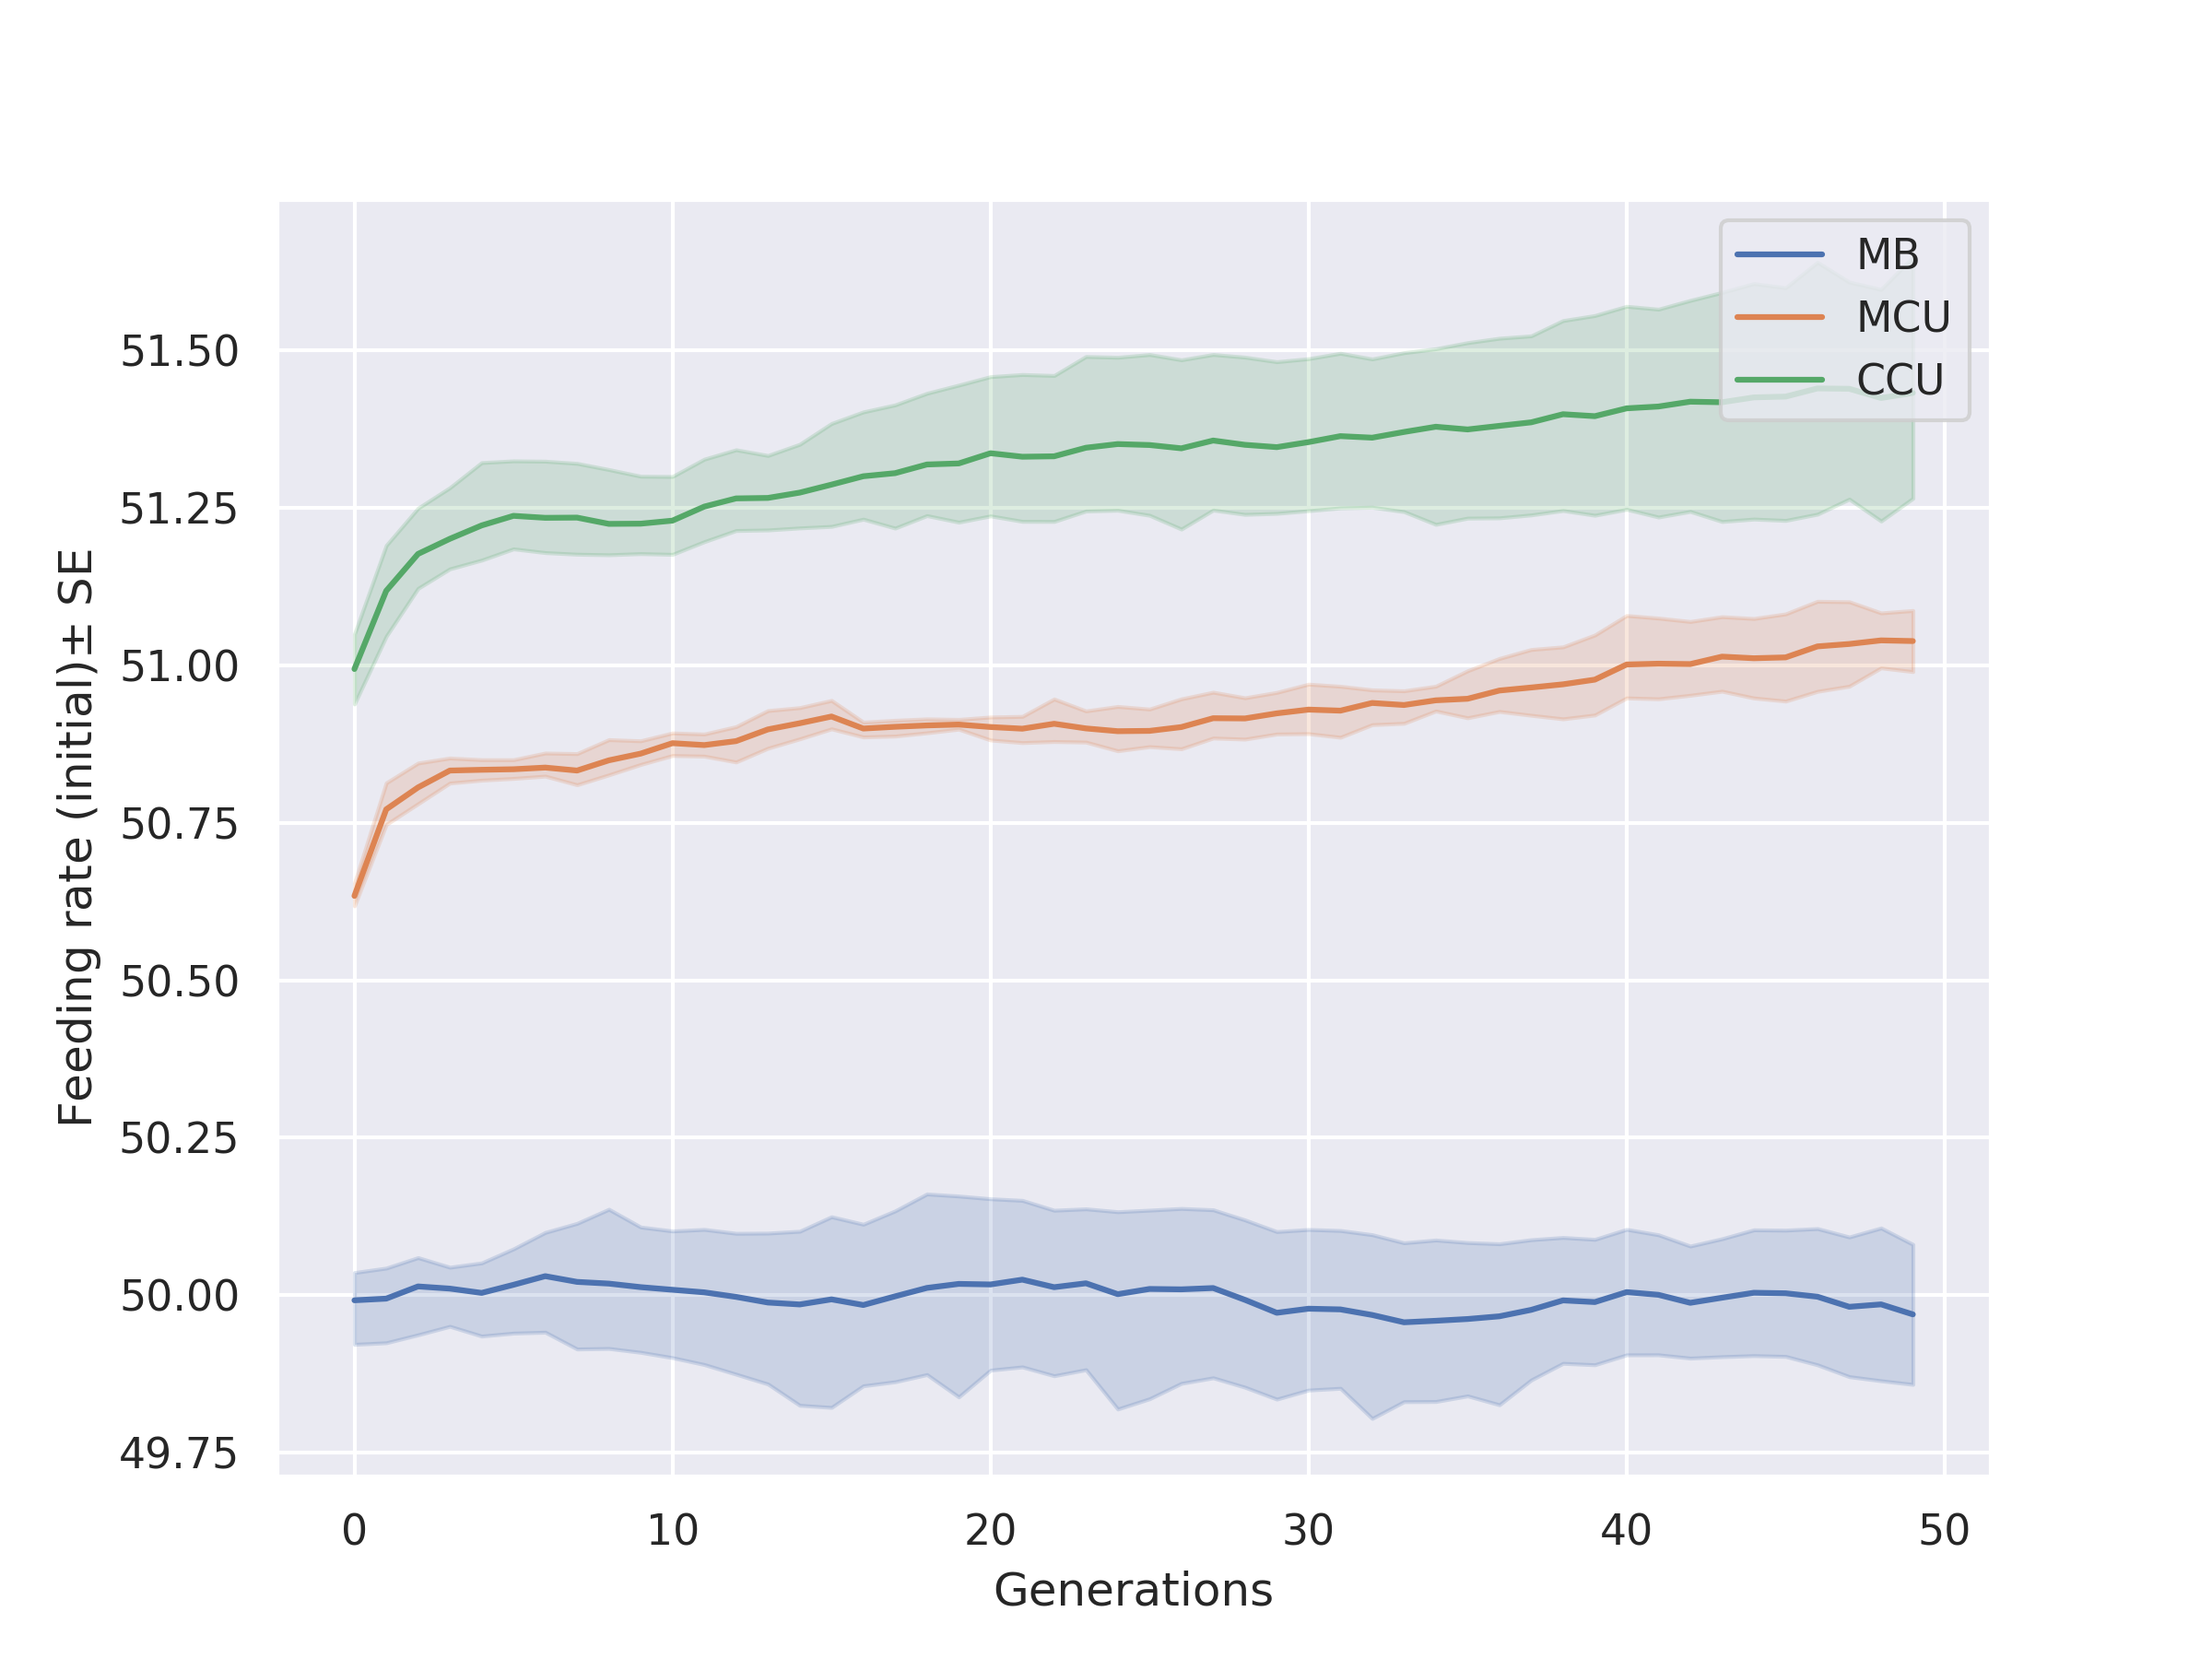
\includegraphics[trim = 0 0 50 50, clip, width=0.75\textwidth]{C4/Figs/fr}
  \caption{Timeseries for initial feeding rate}
  \label{fr}
\end{figure}
\begin{figure}[p]
  \centering
  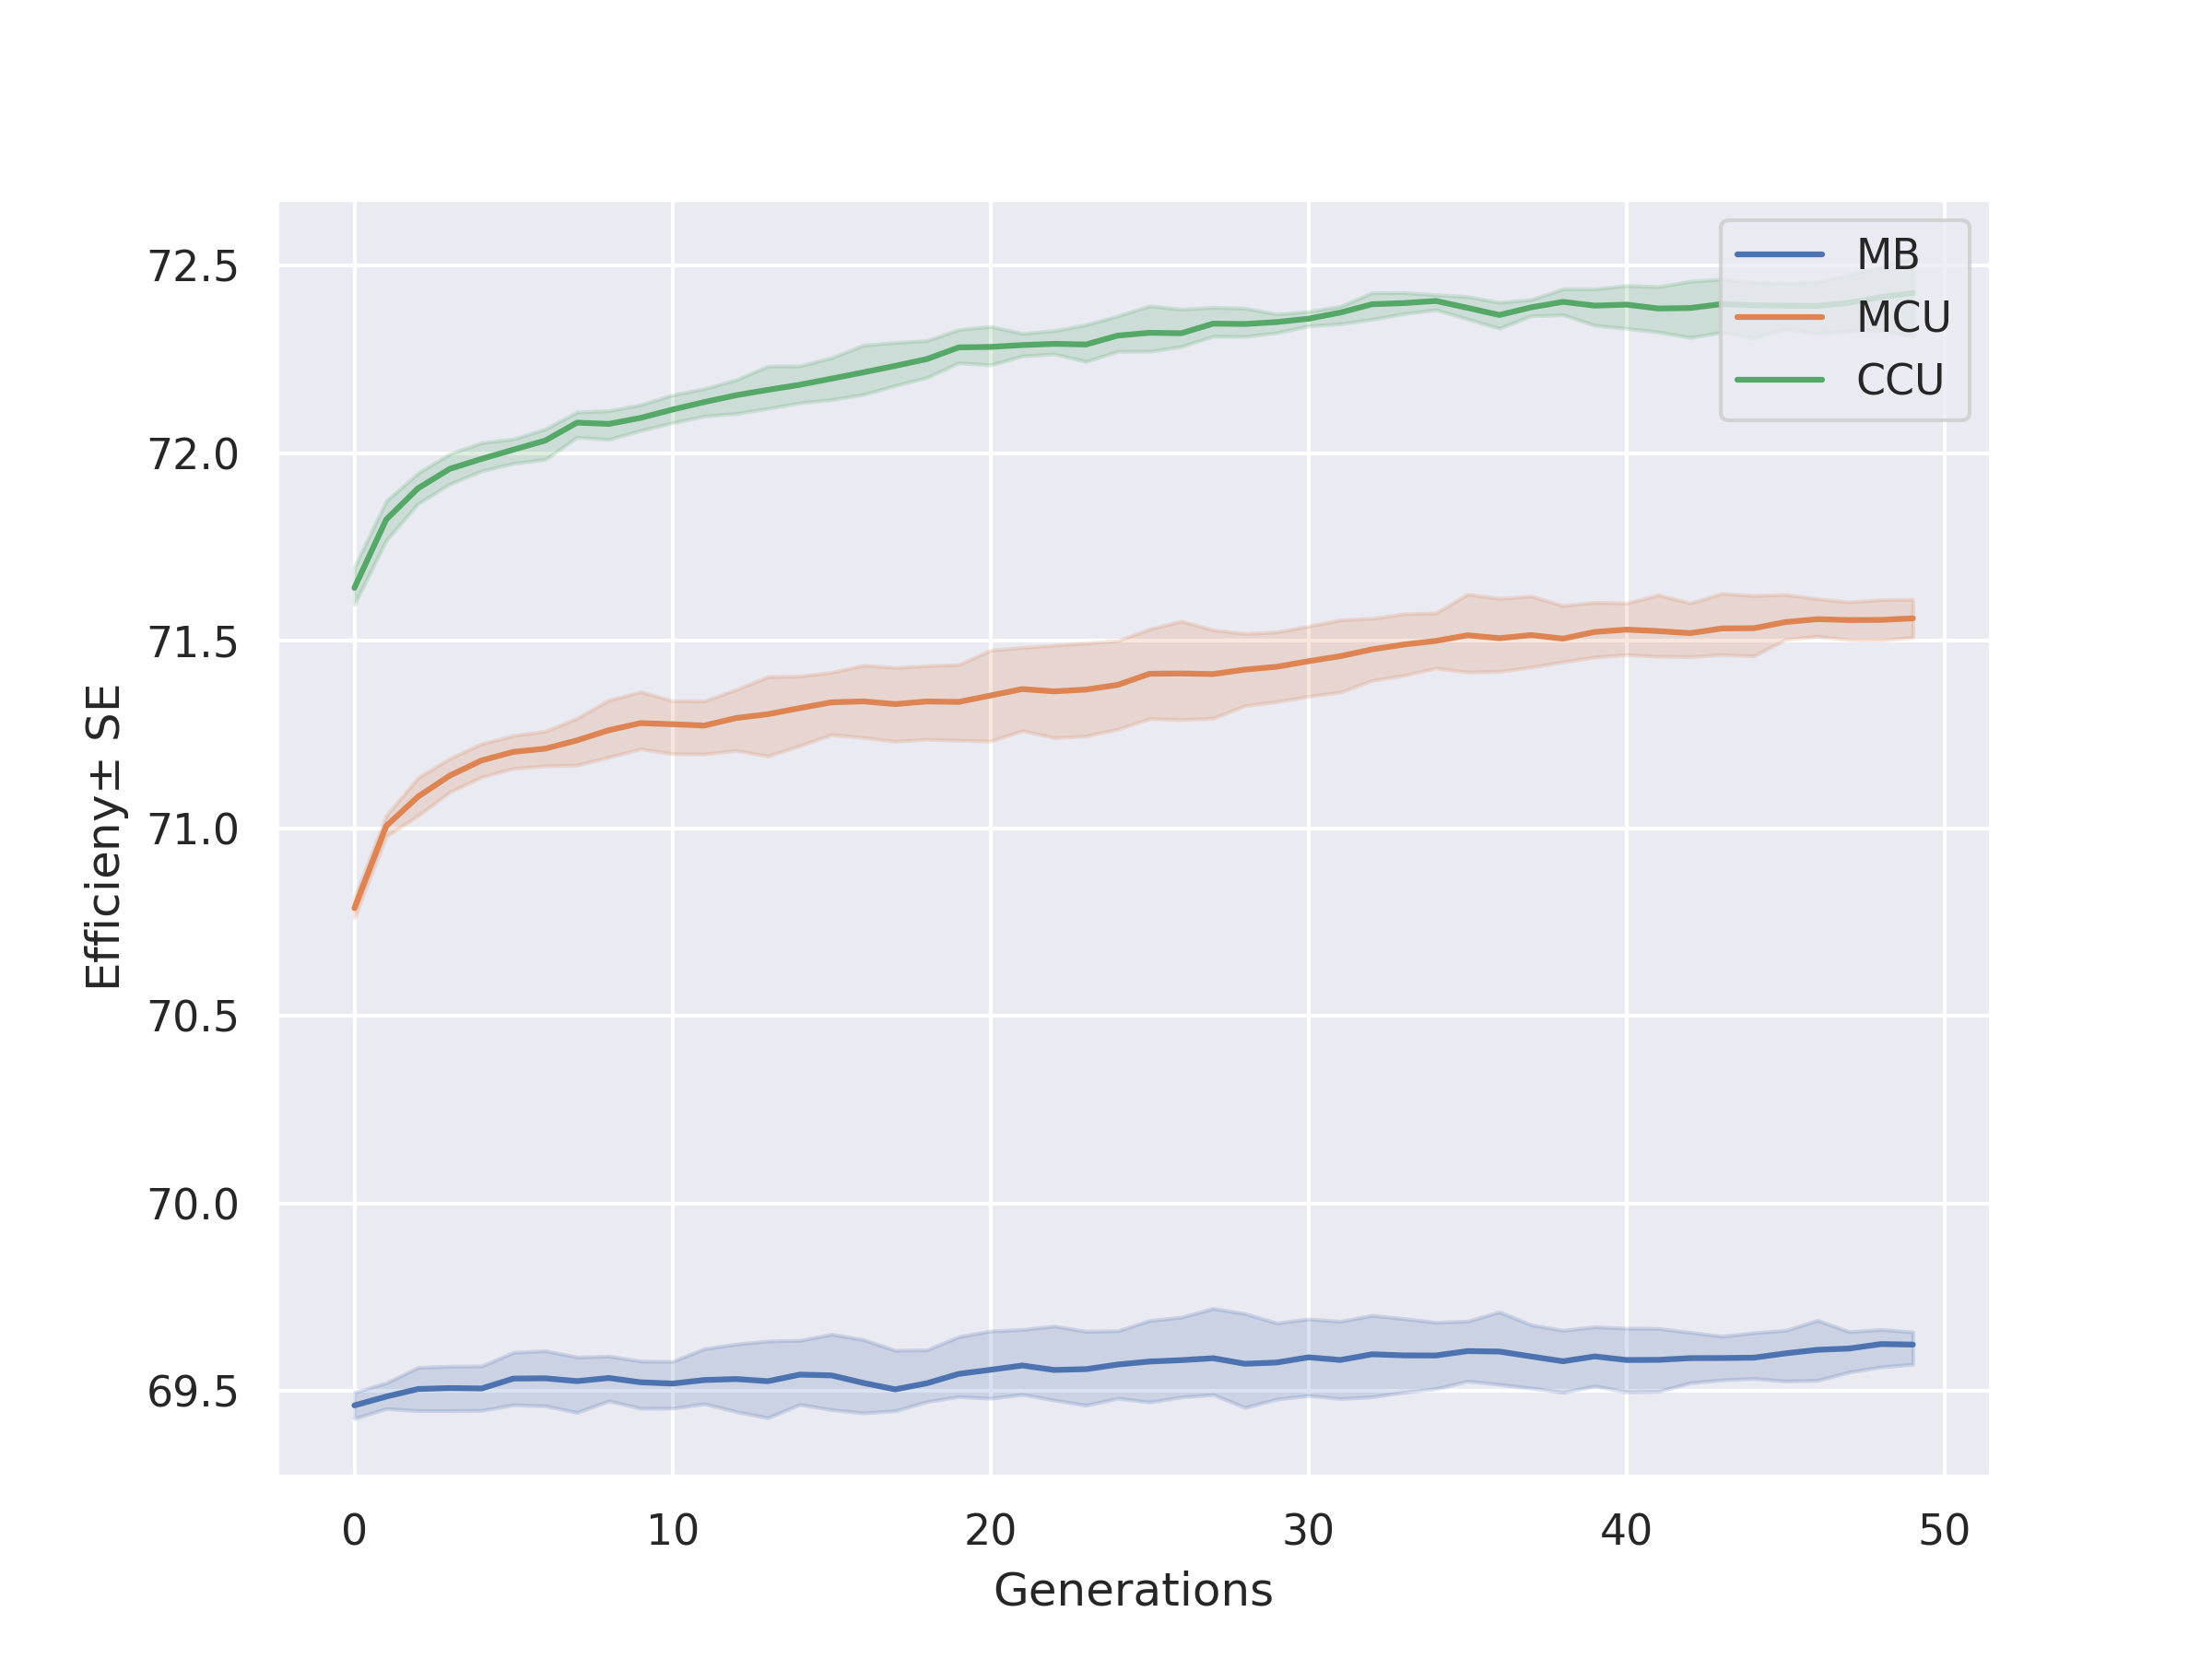
\includegraphics[trim = 0 0 50 50, clip, width=0.75\textwidth]{C4/Figs/eff}
  \caption{Timeseries for efficiency}
  \label{eff}
\end{figure}
\begin{figure}[p]
  \centering
  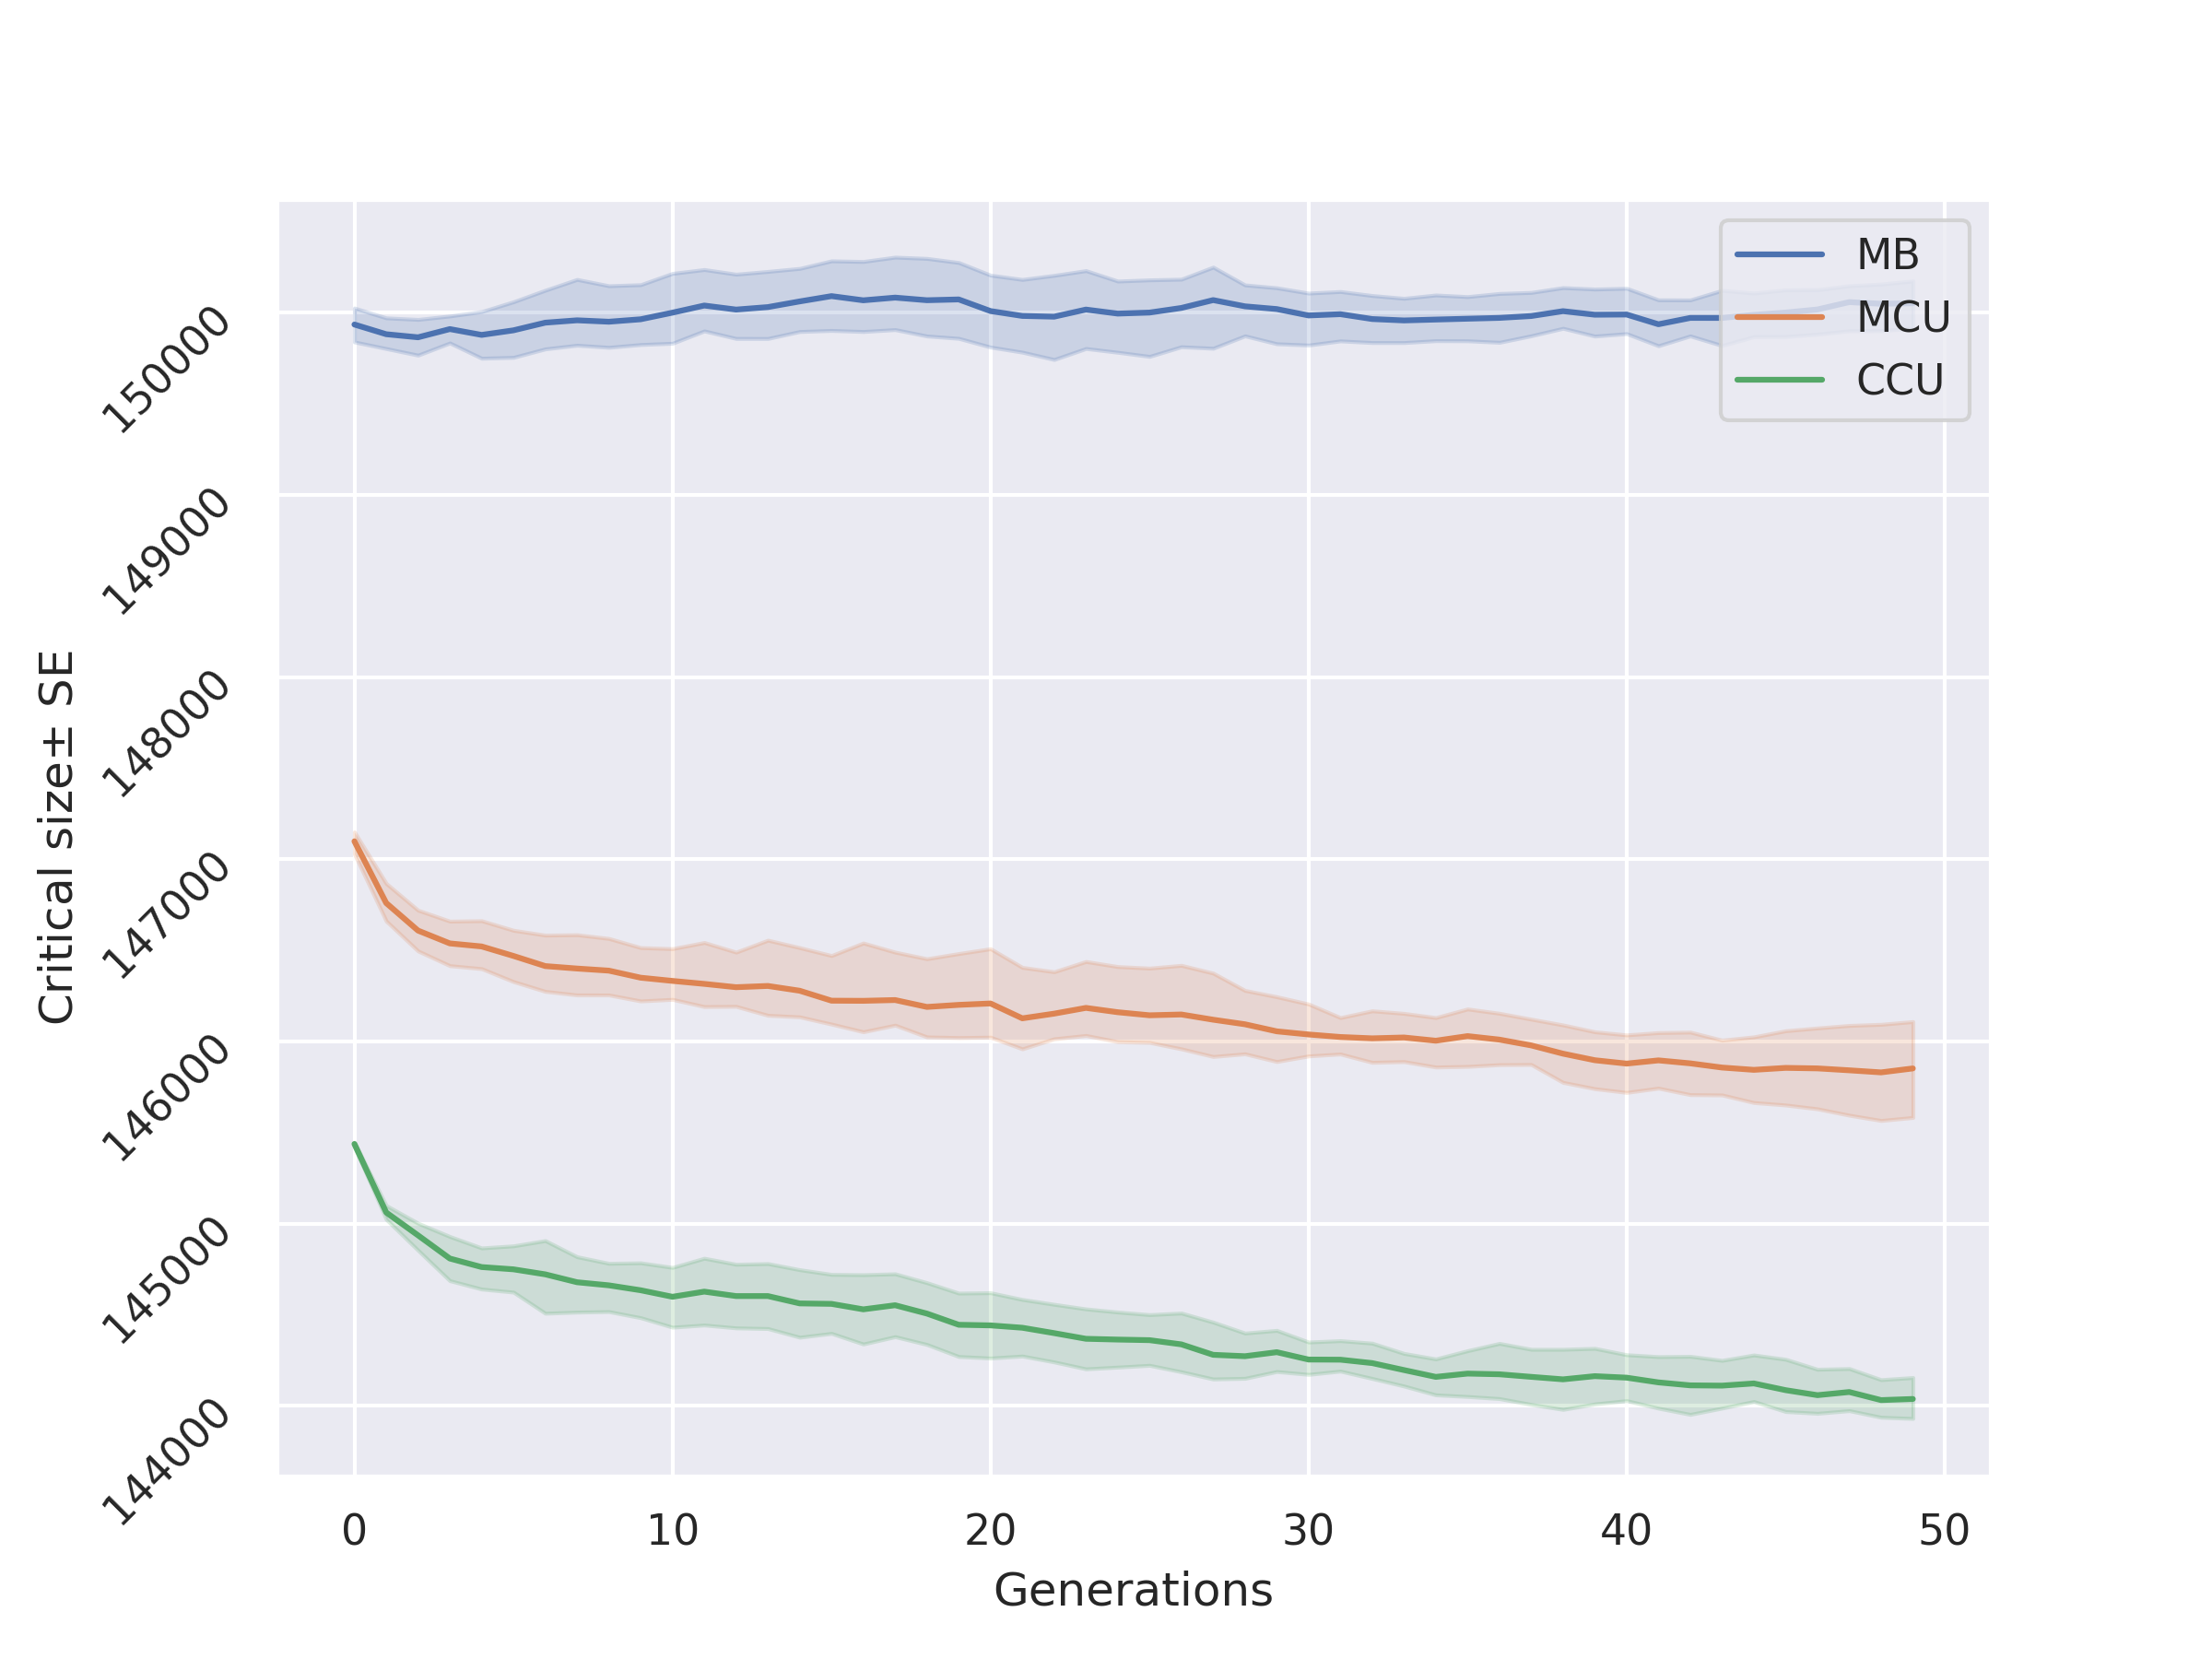
\includegraphics[trim = 0 0 50 50, clip, width=0.75\textwidth]{C4/Figs/mc}
  \caption{Timeseries for critical size}
  \label{mc}
\end{figure}

\clearpage

\begin{figure}[t]
  \centering
  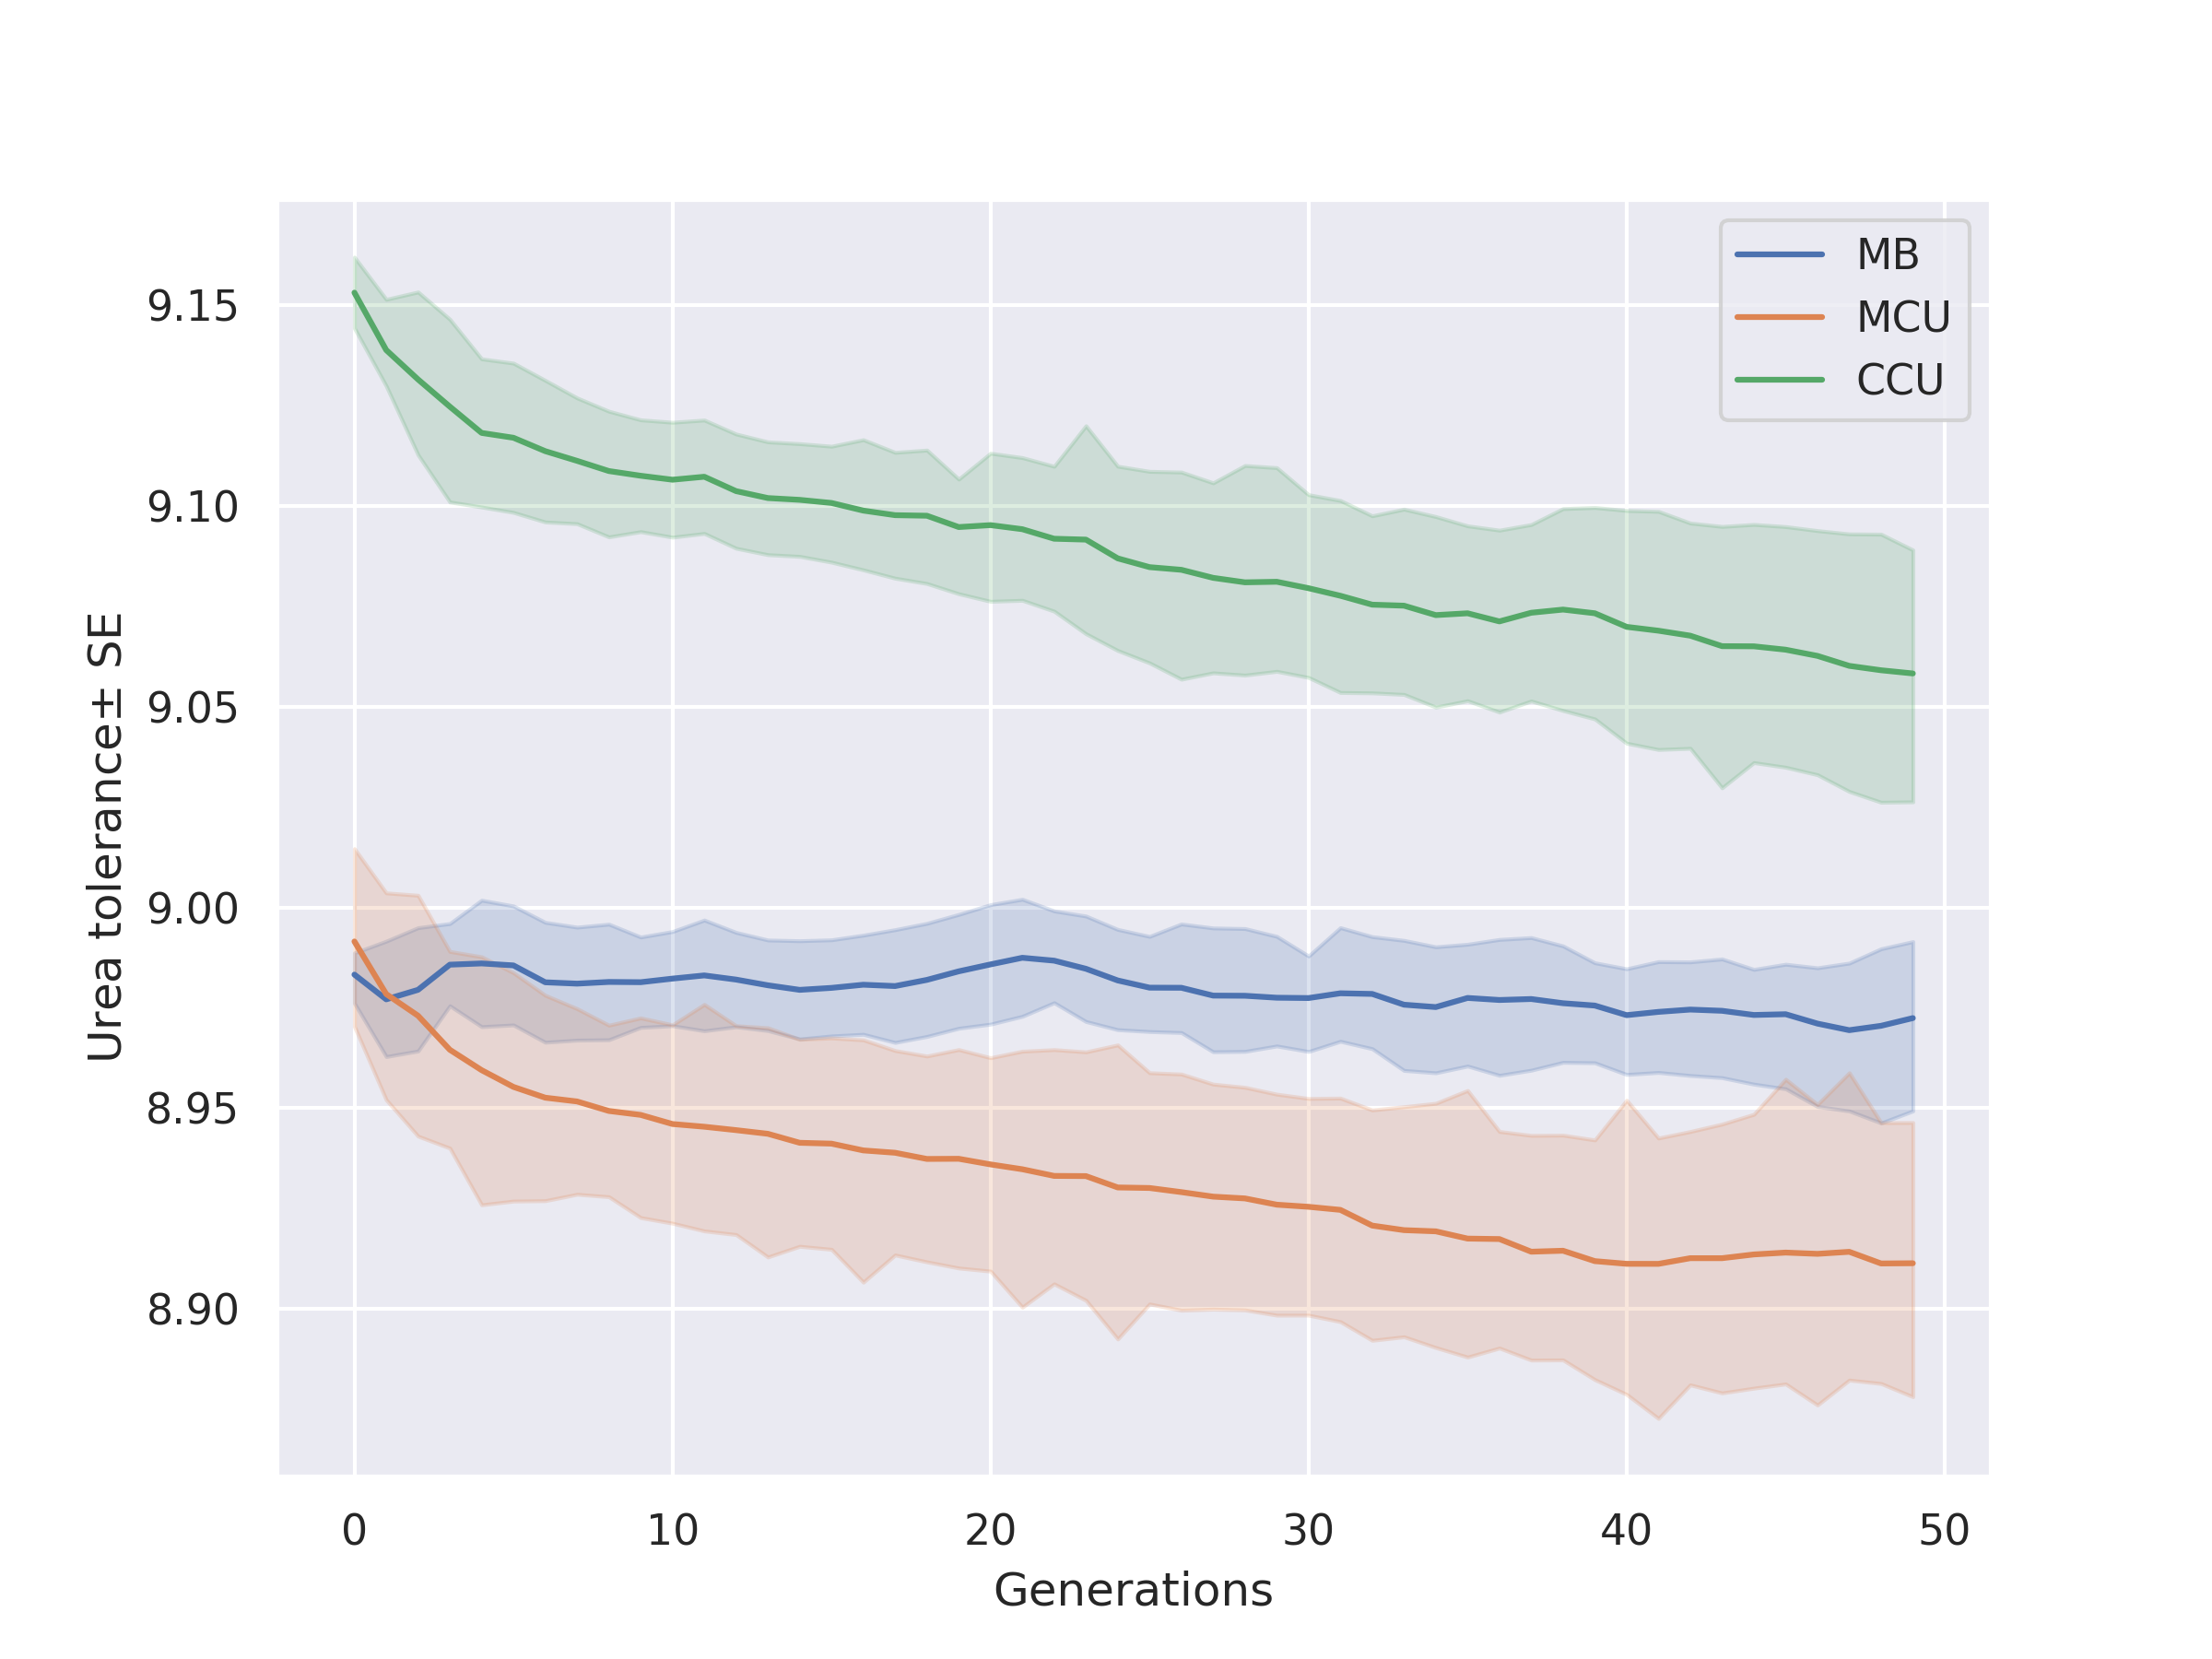
\includegraphics[trim = 0 0 50 50, clip, width=0.75\textwidth]{C4/Figs/wtol}
  \caption{Timeseries for waste tolerance}
  \label{wtol}
\end{figure}
\section{Evolution of Fitness-related Life-history Traits}
From previous simulations on the evolution of larval trait parameters related to competitive ability, mean trait values of above-mentioned larval trait parameters are obtained for MB, MCU and CCU populations after 50 generations. Using mean trait values of initial feeding rate, efficiency, critical size and waste tolerance of respective populations; the larval stage model is simulated in order to investigate the evolution of fitness-related larval traits (replicates = 10). These traits include larval body size, survivorship, and time to reach critical size measured across MB, MCU and CCU culture densities (see fig~\ref{fig:lh-bs} - ~\ref{fig:lh-dt}).\\\\
At higher densities, all fitness-related traits show the effect of larval density. Body size fand survivorship or all three populations is lesser at MCU culture (600 eggs / 1.5 ml) and CCU culture (1200 eggs / 3 ml) (see fig~\ref{fig:lh-bs}). MCU larvae show a larger body size than CCU larvae at low density. Survivorship is higher in MCU culture than in CCU culture for all three populations (see fig~\ref{fig:lh-sur}). Survivorship has increased in MCU and CCU population at high densities, such that CCU larvae survive more than MCU larvae in both MCU and CCU cultures. Time to reach critical size is higher at higher densities for all three populations (see fig~\ref{fig:lh-dt}).\\\\
MCU larvae are able to reach critical size faster than CCU at all densities. Both MCU and CCU larvae reach evolved faster critical feeding time. The majority of these simulation results are similar to the empirical data, except for the survivorship results of CCU larvae \citep{sarangiEcologicalDetailsMediate2018}.
\begin{figure}[h]
  \centering
  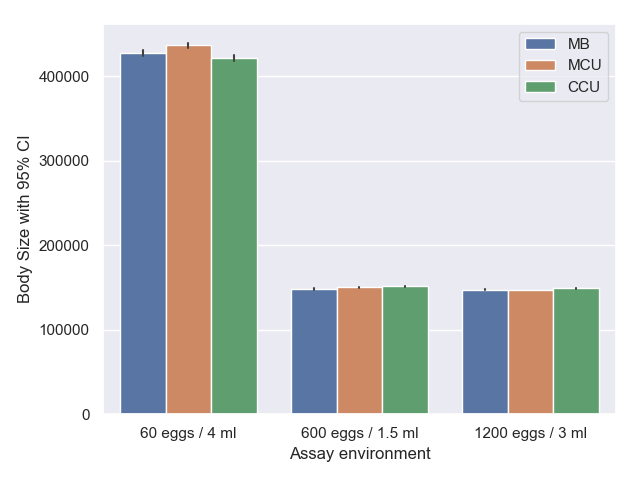
\includegraphics[width=.75\textwidth]{C4/Figs/larval_alive_sizec4}
  \caption{Mean body size of MB, MCU and CCU populations at $50^{th}$ generation in three different larval densities}
  \label{fig:lh-bs}
\end{figure}
\begin{figure}[p]
  \centering
  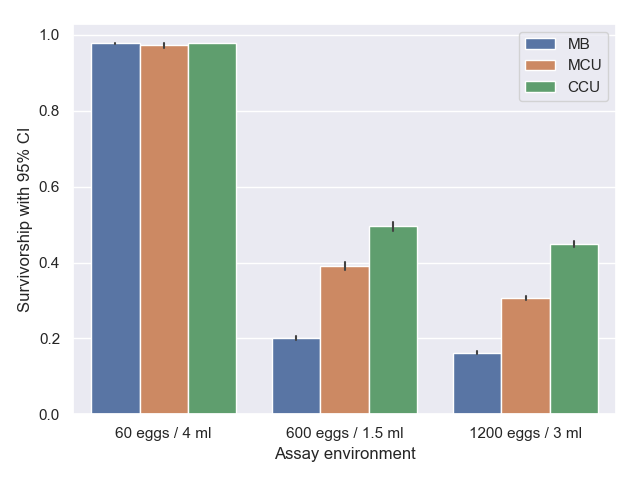
\includegraphics[width=.75\textwidth]{C4/Figs/larval_survc4}
  \caption{Mean survivorship of MB, MCU and CCU populations at $50^{th}$ generation in three different larval densities}
  \label{fig:lh-sur}
\end{figure}
\begin{figure}[p]
  \centering
  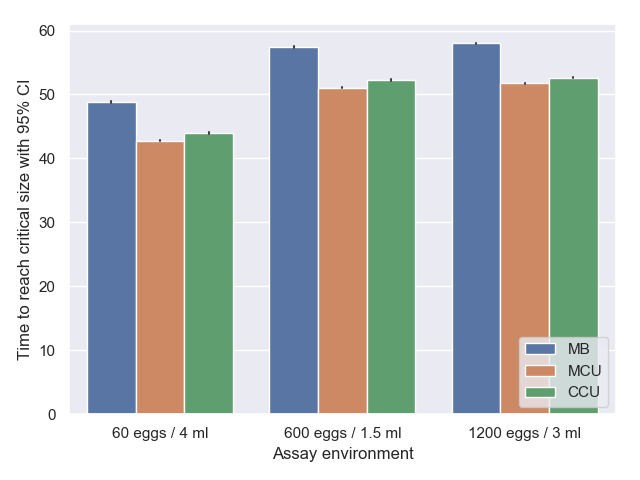
\includegraphics[width=.75\textwidth]{C4/Figs/larval_alive_devtc4}
  \caption{Mean time to reach critical size of MB, MCU and CCU populations at $50^{th}$ generation in three different larval densities}
  \label{fig:lh-dt}
\end{figure}
\pagebreak
